% \documentclass[aspectratio=169,notes]{beamer}
\documentclass[aspectratio=169]{beamer}
\usetheme[faculty=phil]{fibeamer}
\usepackage{polyglossia}
\setmainlanguage{english} %% main locale instead of `english`, you
%% can typeset the presentation in either Czech or Slovak,
%% respectively.
\setotherlanguages{russian} %% The additional keys allow
%%
%%   \begin{otherlanguage}{czech}   ... \end{otherlanguage}
%%   \begin{otherlanguage}{slovak}  ... \end{otherlanguage}
%%
%% These macros specify information about the presentation
\title[MaM]{Mechanics and Machines, Lecture 2} %% that will be typeset on the
\subtitle{Intro to Theory of Mechanisms and Machines
\\ Links, Joints (Kinematic pairs)     \\ Kinematic chains, Degrees of Freedom, Mobility  
         } %% title page.
\author{Oleg Bulichev}
%% These additional packages are used within the document:
\usepackage{ragged2e}  % `\justifying` text
\usepackage{booktabs}  % Tables
\usepackage{tabularx}
\usepackage{tikz}      % Diagrams
\usetikzlibrary{calc, shapes, backgrounds}
\usepackage{amsmath, amssymb}
\usepackage{url}       % `\url`s
\usepackage{listings}  % Code listings
% \usepackage{subfigure}
\usepackage{floatrow}
\usepackage{subcaption}
\usepackage{mathtools}
\usepackage{todonotes}
\usepackage{fontspec}
\usepackage{multicol}
\usepackage{pdfpages}
\usepackage{wrapfig}
\usepackage{animate}
\usepackage{booktabs}
\usepackage{multirow}

\graphicspath{{resources/}}
\frenchspacing

\setbeamertemplate{caption}[numbered]
\usetikzlibrary{graphs}

% \usepackage[backend=biber,style=ieee,autocite=footnote]{biblatex}
% \addbibresource{biblio.bib}
% \DefineBibliographyStrings{english}{%
%   bibliography = {References},}

\newcommand{\oleg}[2][] {\todo[color=red, #1] {OLEG:\\ #2}}
\newcommand{\fbckg}[1]{\usebackgroundtemplate{\includegraphics[width=\paperwidth]{#1}}}%frame background

\usepackage[framemethod=TikZ]{mdframed}
\newcommand{\dbox}[1]{
\begin{mdframed}[roundcorner=3pt, backgroundcolor=yellow, linewidth=0]
\vspace{1mm}
{#1}
\vspace{1mm}
\end{mdframed}
}

\begin{document}
\setlength{\abovedisplayskip}{0pt}
\setlength{\belowdisplayskip}{0pt}
\setlength{\abovedisplayshortskip}{0pt}
\setlength{\belowdisplayshortskip}{0pt}

\fbckg{fibeamer/figs/title_page.png}
\frame[c]{\setcounter{framenumber}{0}
    \usebeamerfont{title}%
    \usebeamercolor[fg]{title}%
    \begin{minipage}[b][6.5\baselineskip][b]{\textwidth}%
        \textcolor{black}{\raggedright\inserttitle}
    \end{minipage}
    % \vskip-1.5\baselineskip

    \usebeamerfont{subtitle}%
    \usebeamercolor[fg]{framesubtitle}%
    \begin{minipage}[b][3\baselineskip][b]{\textwidth}
        \raggedright%
        \insertsubtitle%
    \end{minipage}
    \vskip.25\baselineskip
}
%   \frame[c]{\maketitle}

\fbckg{fibeamer/figs/common.png}

\note{\scriptsize \begin{itemize}
    \item \ 
\end{itemize}}

\begin{frame}[t]{Mechanisms and their elements}
\framesubtitle{Terminology}
    \begin{block}{Mechanism}
        It's an artificially created system of bodies designed to transform the movement of one or several bodies into the required movements of other bodies.
    \end{block}
    \begin{exampleblock}{Link}
        Rigid body
    \end{exampleblock}
    \begin{block}{Joint}
        A permanent contact (connection) between two links.
    \end{block}
\end{frame}



\begin{frame}[t]{Degrees of Freedom}
    \framesubtitle{Video}
    \vspace{-0.6cm}
    \begin{figure}[H]
        \href{https://youtu.be/zI64DyaRUvQ}{
            \centering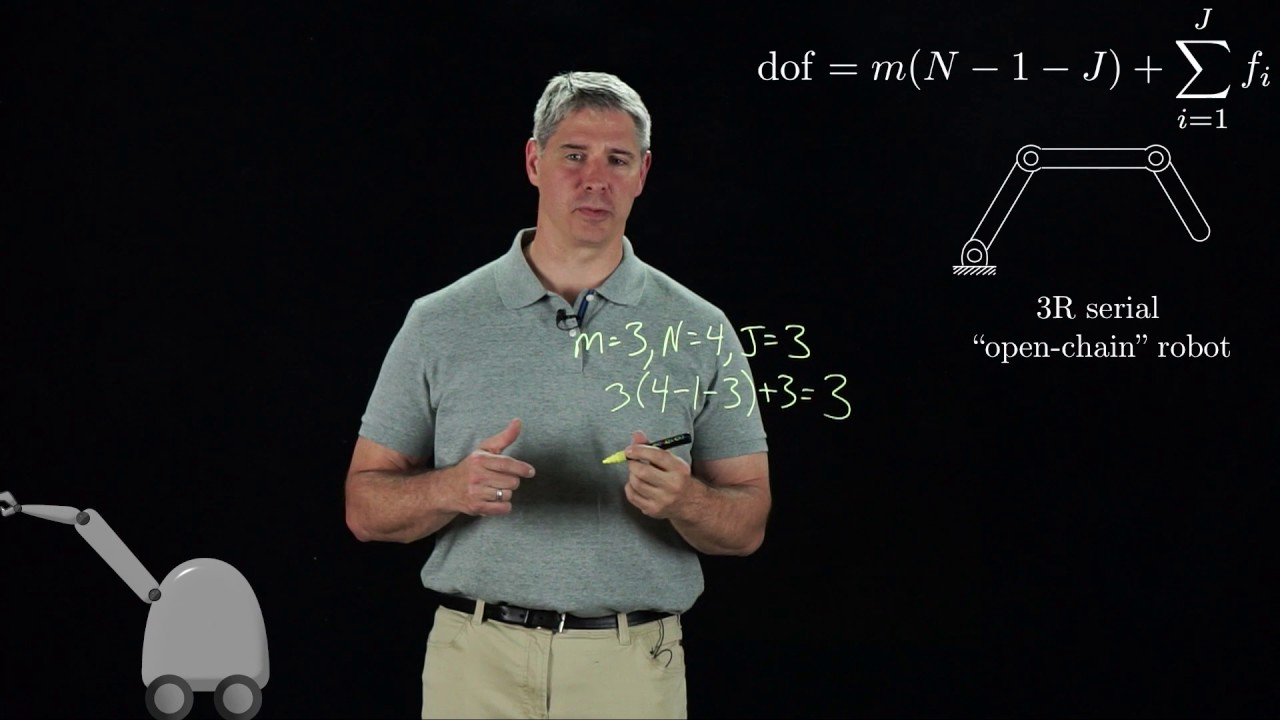
\includegraphics[height=6cm,width=1\textwidth,keepaspectratio]{dof_video.jpg}}
        % \caption{Click on a picture for a video}
        \label{fig:dof_video.jpg}
    \end{figure}
\end{frame}


\begin{frame}[t]{Reference material}
    % \Large
    \begin{itemize}
        \item \textit{"Mechanisms and Machines: Kinematics, Dynamics, and Synthesis" Michael M. Stanisic, pdf pages 21--56 } \textbf{1.1 --- 1.6}
        \item \textit{"Theory of Machines and Mechanisms" John J. Uicker, pdf pages 33--59 } \textbf{1.4 --- 1.7}
        \item \textit{"Design of machinery" Robert L. Norton, pdf pages 57--79 } \textbf{2.0 --- 2.11}
        \item \textit{"Механика. Теория механизмов и машин" Конищева О. В., pdf pages 7--23 } \\ Структурный анализ и классификация плоских механизмов
        \item \textit{"Теория механизмов и машин" Артоболевский И. И. 1988, pdf pages 21--63 } \\ Структурный анализ и классификация механизмов
        % \item \href{https://onlinemschool.com/math/library/vector/cos/}{Direction cosines (OnlineMSchool)}
    \end{itemize}
\end{frame}

\fbckg{fibeamer/figs/last_page.png}
\frame[plain]{}

\end{document}